\section{Results}
\label{sec:results}

All estimates are selective five-label Hamming error at the frozen
\SI{80}{\percent} coverage cutoff, with \SI{95}{\percent} percentile intervals
from a patient-clustered bootstrap of \num{2000} replicates. Thresholds and
abstention cutoffs are the source-site values applied unchanged at both sites.
This section reports what was estimated; interpretation is deferred to
\cref{sec:discussion}.

\begin{figure}[tbp]
\centering
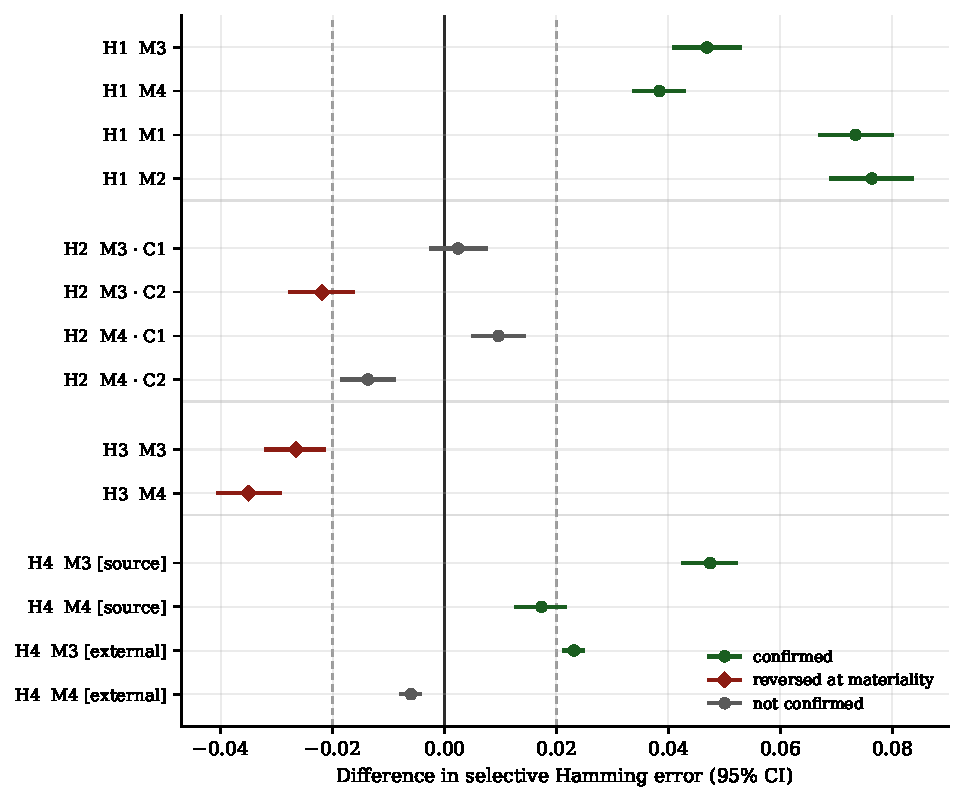
\includegraphics[width=\linewidth]{figures/fig1_forest}
\caption{Confirmatory contrasts with \SI{95}{\percent} percentile intervals
from the patient-clustered bootstrap. Dashed lines mark the materiality
threshold of $\pm\num{0.02}$. Two contrasts are reversed: their intervals
exclude zero on the side opposite the prediction, with magnitudes exceeding
materiality.}
\label{fig:forest}
\end{figure}

\cref{fig:forest} summarises the four confirmatory contrasts; the
subsections below give the estimates.

\subsection{Cohorts}

The source confirmatory tier comprises \num{16456} images from \num{14766}
studies and \num{5000} patients. Every study is informative (N1) by
construction, since cohort selection already required context above the frozen
threshold.

The external cohort comprises \num{191070} usable images from \num{187673}
studies and \num{64709} patients, one image having been excluded as corrupt in
the published dataset. Here the natural-state distribution is informative:
\num{132923} studies (\SI{70.8}{\percent}) are N1, \num{14129}
(\SI{7.5}{\percent}) are N2, and \num{40622} (\SI{21.6}{\percent}) are N3.
Interventions therefore apply to \num{132923} external studies against
\num{14766} source studies.

Invariants held at both sites. Image-only predictions were identical across all
three context conditions (maximum drift \num{0}), and studies retaining their
own context under C2 numbered \num{6} of \num{14766} at the source site and
\num{34} of \num{132923} at the external site.

\subsection{Selective risk at both sites}

\begin{table}[htbp]
\centering
\caption{Selective Hamming error at the frozen \SI{80}{\percent} cutoff. M1 is
image-only, M2 text-only, M3 probability late fusion, M4 feature-concatenation
fusion. M1 is invariant to the context intervention by construction.}
\label{tab:selective-risk}
\begin{tabular}{lccc c ccc}
\toprule
& \multicolumn{3}{c}{Source site} & & \multicolumn{3}{c}{External site} \\
\cmidrule{2-4}\cmidrule{6-8}
Model & C0 & C1 & C2 & & C0 & C1 & C2 \\
\midrule
M1 & 0.1084 & 0.1084 & 0.1084 & & 0.1818 & 0.1818 & 0.1818 \\
M2 & 0.1575 & 0.2411 & 0.2415 & & 0.2338 & 0.2605 & 0.2667 \\
M3 & 0.1102 & 0.0951 & 0.1426 & & 0.1570 & 0.1444 & 0.1676 \\
M4 & \textbf{0.0744} & 0.0720 & 0.0893 & & \textbf{0.1128} & 0.1200 & 0.1140 \\
\bottomrule
\end{tabular}
\end{table}

M4 attains the lowest selective error under every site-by-condition
combination (\cref{fig:risk}).

\begin{figure}[htbp]
\centering
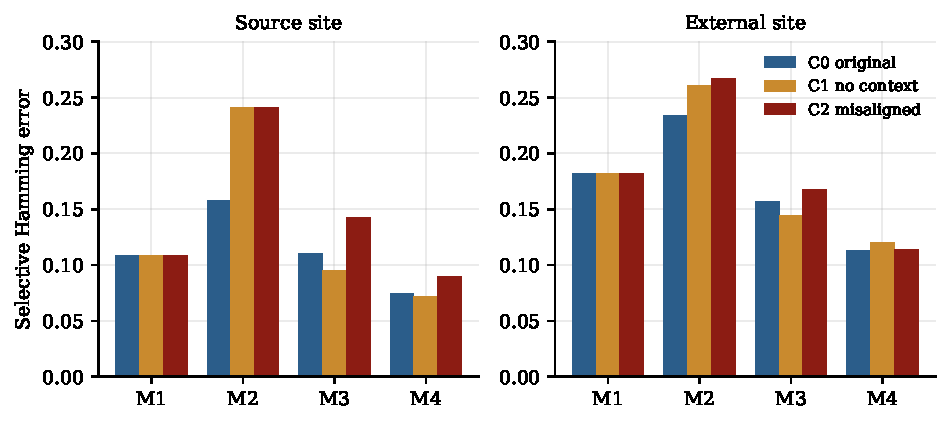
\includegraphics[width=\linewidth]{figures/fig2_risk}
\caption{Selective Hamming error at the frozen \SI{80}{\percent} cutoff.
Every model degrades on institutional transfer; the ordering between models is
preserved.}
\label{fig:risk}
\end{figure}


\subsection{H1: transport of the selective policy}

\begin{table}[htbp]
\centering
\caption{H1, external minus source selective error under intact context (C0).
M3 and M4 are the confirmatory models; M1 and M2 are reported for context.}
\label{tab:h1}
\begin{tabular}{lccl}
\toprule
Model & Estimate & \SI{95}{\percent} CI & Verdict \\
\midrule
M3 & $+0.0469$ & $(+0.0408,\ +0.0531)$ & \textbf{confirmed} \\
M4 & $+0.0384$ & $(+0.0336,\ +0.0430)$ & \textbf{confirmed} \\
\midrule
M1 & $+0.0734$ & $(+0.0668,\ +0.0802)$ & confirmed \\
M2 & $+0.0763$ & $(+0.0687,\ +0.0838)$ & confirmed \\
\bottomrule
\end{tabular}
\end{table}

H1 is confirmed for both confirmatory models. Every interval excludes zero in
the hypothesised direction and every point estimate exceeds the materiality
threshold of \num{0.02}, by factors of \numrange{1.9}{3.8}. These estimates are
taken under C0, with context intact at both sites.

\subsection{H2: compound interaction}

\begin{table}[htbp]
\centering
\caption{H2, the interaction between institutional and context shift, computed
as the context effect at the external site minus the same effect at the source
site. A positive value would indicate super-additivity.}
\label{tab:h2}
\begin{tabular}{llcl}
\toprule
Model & Condition & Estimate & \SI{95}{\percent} CI \\
\midrule
M3 & C1 & $+0.0024$ & $(-0.0027,\ +0.0076)$ \\
M3 & C2 & $-0.0219$ & $(-0.0279,\ -0.0160)$ \\
M4 & C1 & $+0.0096$ & $(+0.0048,\ +0.0144)$ \\
M4 & C2 & $-0.0137$ & $(-0.0185,\ -0.0087)$ \\
\bottomrule
\end{tabular}
\end{table}

H2 is not confirmed in any of its four instances. One estimate is
indistinguishable from zero (M3 under C1). Two exclude zero in the direction
opposite to the hypothesis (M3 and M4 under C2), and for M3 the magnitude
reaches materiality, so the effect is reversed rather than absent. The
remaining estimate excludes zero in the hypothesised direction but falls below
materiality (M4 under C1, $+0.0096$).

\subsection{H3: multimodal versus image-only exposure}

\begin{table}[htbp]
\centering
\caption{H3, the transfer gap of each multimodal model minus the transfer gap of
the image-only control. A positive value would indicate greater multimodal
exposure.}
\label{tab:h3}
\begin{tabular}{lccl}
\toprule
Contrast & Estimate & \SI{95}{\percent} CI & Verdict \\
\midrule
M3 $-$ M1 & $-0.0265$ & $(-0.0321,\ -0.0212)$ & reversed at materiality \\
M4 $-$ M1 & $-0.0350$ & $(-0.0408,\ -0.0292)$ & reversed at materiality \\
\bottomrule
\end{tabular}
\end{table}

H3 is not confirmed, and the direction is reversed for both models. Each
interval lies entirely below zero, and each magnitude exceeds materiality.
Both multimodal models carry smaller transfer gaps than the image-only control.
The advantage of M4 over M1 in absolute selective error also widens across
sites, from \num{0.034} at the source site to \num{0.069} at the external site.

\subsection{H4: conflicting versus absent context}

\begin{table}[htbp]
\centering
\caption{H4, C2 minus C1 within site. A non-negative value indicates that
misaligned context is no better than absent context.}
\label{tab:h4}
\begin{tabular}{llccl}
\toprule
Site & Model & Estimate & \SI{95}{\percent} CI & Verdict \\
\midrule
Source   & M3 & $+0.0475$ & $(+0.0422,\ +0.0524)$ & confirmed \\
Source   & M4 & $+0.0173$ & $(+0.0125,\ +0.0217)$ & confirmed \\
External & M3 & $+0.0231$ & $(+0.0211,\ +0.0250)$ & confirmed \\
External & M4 & $-0.0060$ & $(-0.0080,\ -0.0041)$ & not confirmed \\
\bottomrule
\end{tabular}
\end{table}

H4 holds in three of four instances. The exception is M4 at the external site,
where the estimate is negative and its interval excludes zero, but the
magnitude is below materiality.

\subsection{Coverage under the frozen cutoff}

A coverage drift of \num{0.05} from the \SI{80}{\percent} target was
prespecified as material. Under intact context, no model breaches it at either
site; the largest external departure is M2 at $+0.0469$ and the smallest is M4
at $-0.0051$.

Four breaches occur, all under context intervention and all at both sites
alike:

\begin{itemize}
  \item M2 under C1 reaches \SI{100}{\percent} coverage at both sites
    (drift $+0.20$). Replacing every context with a single placeholder makes the
    text-only model's output constant, so all studies clear the confidence
    cutoff simultaneously.
  \item M3 under C2 falls to \SI{72.8}{\percent} at the source site
    (drift $-0.0718$) and \SI{74.6}{\percent} at the external site
    (drift $-0.0537$).
\end{itemize}

M4's coverage remains within \num{0.036} of target under every site-by-condition
combination.

\begin{figure}[htbp]
\centering
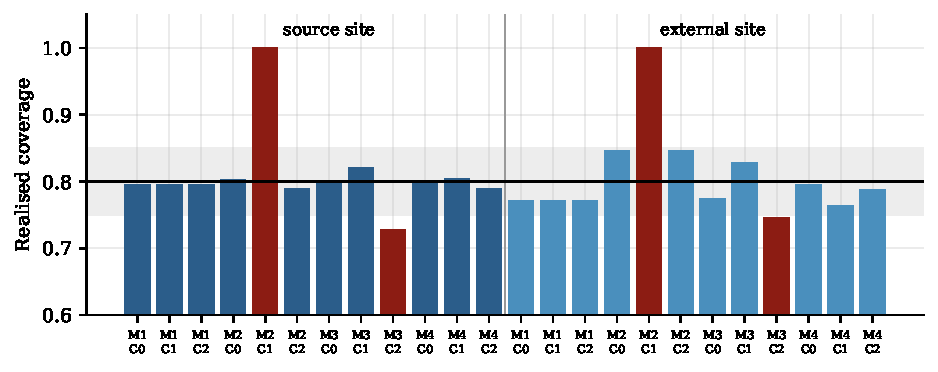
\includegraphics[width=\linewidth]{figures/fig3_coverage}
\caption{Realised coverage under the frozen cutoff. The shaded band marks the
prespecified material drift of \num{0.05} either side of the
\SI{80}{\percent} target; bars breaching it are darkened. Coverage survives
institutional transfer and fails under context intervention.}
\label{fig:coverage}
\end{figure}

\subsection{Coverage sensitivity}

Coverages of \SI{90}{\percent} and \SI{70}{\percent} were pre-specified as
sensitivity analyses alongside the primary \SI{80}{\percent}.

\begin{table}[htbp]
\centering
\caption{Point estimates for the two confirmatory contrasts across the three
pre-specified coverages. H1 is the transfer gap under intact context; H3 is that
gap minus the image-only control's.}
\label{tab:coverage-sensitivity}
\begin{tabular}{llccc}
\toprule
& Model & \SI{70}{\percent} & \SI{80}{\percent} & \SI{90}{\percent} \\
\midrule
\multirow{2}{*}{H1} & M3 & $+0.0394$ & $+0.0469$ & $+0.0548$ \\
                    & M4 & $+0.0392$ & $+0.0384$ & $+0.0374$ \\
\midrule
\multirow{2}{*}{H3} & M3 & $-0.0296$ & $-0.0265$ & $-0.0234$ \\
                    & M4 & $-0.0299$ & $-0.0350$ & $-0.0408$ \\
\bottomrule
\end{tabular}
\end{table}

Both conclusions hold across all three coverages. Every H1 estimate remains
positive and above materiality, and every H3 estimate remains negative and above
materiality in magnitude, so neither the confirmation nor the reversal depends on
the choice of operating point. The two multimodal models respond to coverage in
opposite directions --- M3's transfer gap grows with coverage while M4's shrinks
--- but not enough to alter either verdict.

\subsection{Informativeness-threshold sensitivity}
\label{sec:threshold-sensitivity}

A study enters the intervention cohort as N1 only if its pre-diagnostic context
carries at least $T$ effective tokens. $T = 3$ was pre-specified as primary;
$T = 5$ and $T = 10$ were pre-specified as sensitivities. The threshold is a
cohort definition rather than a model setting, so raising it does not merely
perturb an estimate --- it re-runs the whole evaluation on a smaller and more
text-rich population. At the external site the N1 cohort falls from
\num{132923} studies at $T = 3$ to \num{111040} at $T = 5$ and \num{23146} at
$T = 10$, the last retaining under a fifth of the primary cohort; at the source
site it falls from \num{14766} to \num{13600} and \num{8381}. Studies leaving N1
become N2, so the comparison is between populations, not nested subsamples of
one.

\begin{table}[htbp]
\centering
\caption{Point estimates for the two confirmatory contrasts across the three
pre-specified informativeness thresholds, at \SI{80}{\percent} coverage. H1 is
the transfer gap under intact context; H3 is that gap minus the image-only
control's.}
\label{tab:threshold-sensitivity}
\begin{tabular}{llccc}
\toprule
& Model & $T = 3$ & $T = 5$ & $T = 10$ \\
\midrule
\multirow{2}{*}{H1} & M3 & $+0.0469$ & $+0.0381$ & $+0.0221$ \\
                    & M4 & $+0.0384$ & $+0.0330$ & $+0.0232$ \\
\midrule
\multirow{2}{*}{H3} & M3 & $-0.0265$ & $-0.0314$ & $-0.0338$ \\
                    & M4 & $-0.0350$ & $-0.0366$ & $-0.0327$ \\
\bottomrule
\end{tabular}
\end{table}

All fourteen contrasts --- the four confirmatory ones and the ten secondary and
descriptive ones --- return the same verdict at every threshold. Both H1
estimates stay positive and above materiality, and both H3 estimates stay
negative and above materiality in magnitude, so neither the confirmation of H1
nor the reversal of H3 depends on where the informativeness cut is placed.

The two hypotheses respond to the threshold in opposite directions, and the
direction is interpretable. H1's transfer gap shrinks as $T$ rises, roughly
halving for M3 between $T = 3$ and $T = 10$: restricting the cohort to studies
with substantial context reduces, but does not remove, the penalty for moving
sites. H3's reversal instead deepens slightly, so the multimodal models'
advantage over the image-only control is not an artifact of admitting
thin-context studies that the fusion models handle better than M1 does.

One interval changes character without changing a verdict. H4 for M4 at the
external site is $-0.0060$ (\SI{95}{\percent} CI \numrange{-0.0080}{-0.0041}) at
$T = 3$ but $-0.0020$ ($-0.0067$ to $+0.0023$) at $T = 10$, crossing zero as the
cohort shrinks to \num{23146} studies. The verdict is unaffected because the
estimate falls far short of the \num{0.02} materiality threshold at every $T$
and was never confirmed, but the widening is the expected consequence of a
five-fold smaller cohort and is reported rather than suppressed.

\subsection{S1: cross-site contrasts are not label-invariant}
\label{sec:s1}

The findings-derived label source was pre-specified as a mandatory sensitivity.
It did not perturb the primary estimates; it reversed every contrast that
compares the two sites while leaving every contrast computed within a site
intact. That dissociation is the result of this section. It localises the
instability to the site comparison itself rather than to the models, the
images, or the context intervention, and \cref{sec:comparability} identifies
its cause.

The sensitivity was run end to end: thresholds re-selected on the findings
calibration labels, both sites re-evaluated, and the same bootstrap applied. The
cohort is smaller because findings sections are less often present ---
\num{9293} source evaluation studies against \num{14766}.

\begin{table}[htbp]
\centering
\caption{S1 against the primary. Within-site and between-model contrasts agree;
the two cross-site contrasts do not.}
\label{tab:s1}
\begin{tabular}{llccl}
\toprule
H & Contrast & Primary & S1 (findings) & Agreement \\
\midrule
H1 & M3 external $-$ source & $+0.0469$ & $-0.1324$ & \textbf{reverses} \\
H1 & M4 external $-$ source & $+0.0384$ & $-0.1079$ & \textbf{reverses} \\
H1 & M1 external $-$ source & $+0.0734$ & $-0.0672$ & \textbf{reverses} \\
H1 & M2 external $-$ source & $+0.0763$ & $-0.2385$ & \textbf{reverses} \\
H2 & M3 interaction, C1     & $+0.0024$ & $+0.0340$ & changes verdict \\
H2 & M4 interaction, C1     & $+0.0096$ & $+0.0625$ & changes verdict \\
H3 & M3 $-$ M1 transfer gap & $-0.0265$ & $-0.0652$ & agrees \\
H3 & M4 $-$ M1 transfer gap & $-0.0350$ & $-0.0408$ & agrees \\
H4 & M3 source, C2 $-$ C1   & $+0.0475$ & $+0.0606$ & agrees \\
H4 & M4 source, C2 $-$ C1   & $+0.0173$ & $+0.0479$ & agrees \\
H4 & M3 external, C2 $-$ C1 & $+0.0231$ & $+0.0089$ & agrees \\
H4 & M4 external, C2 $-$ C1 & $-0.0060$ & $-0.0104$ & agrees \\
\bottomrule
\end{tabular}
\end{table}

\textbf{H1 reverses under the sensitivity endpoint.} Under findings-derived
labels the external site shows \emph{lower} selective error than the source
site, by \num{0.13} for M3 and \num{0.11} for M4, with intervals excluding zero.
H2 also changes verdict. H3 and H4 agree in all eight instances.

The pattern separates cleanly by contrast type. Every contrast that compares
across sites changes; every contrast that compares models or conditions within a
site holds.

The image-only control settles what is driving this. M1 consumes no text, and at
the external site its cohort is unchanged between the two runs, so it produces
bit-identical predictions under both label sources (mean study probability
\num{0.603719} in each). Its transfer gap nonetheless reverses, from $+0.0734$
to $-0.0672$. A quantity computed from unchanged predictions cannot have changed
sign because of the models, the images, or the context. Only the labels differ.

The consequence is narrower than a failed replication and wider than a caveat.
It is not that the primary H1 estimate is unstable under resampling --- the
coverage and threshold sensitivities in
\cref{tab:coverage-sensitivity,tab:threshold-sensitivity} show it is not. It is
that a cross-site selective-error contrast is defined only relative to a label
source, and the two label sources compared here are not measuring the same
quantity at the two sites. Any cross-site claim in this paper, in either
direction, is therefore conditional on its endpoint. We report both endpoints
rather than nominating the one that agrees with our hypothesis, and
\cref{sec:comparability} shows the two label sets are not commensurable enough
for either to arbitrate the other.

\subsection{Label-set comparability across sites}
\label{sec:comparability}

The protocol required label distributions be compared site-to-site before the
cross-site experiment, and designated the findings endpoint a sensitivity rather
than a primary on the stated grounds that it is sparse. That comparison explains
the divergence in \cref{tab:s1}.

\begin{table}[htbp]
\centering
\caption{Label-set composition by site and source, evaluation cohorts under C0.
Supervised-cell density is the fraction of study-by-pathology cells carrying a
label at all; positive rate is computed among those cells. Under the primary
endpoint the two sites are closely matched. Under the sensitivity endpoint they
are not.}
\label{tab:comparability}
\begin{tabular}{lcccc}
\toprule
& \multicolumn{2}{c}{Supervised-cell density} & \multicolumn{2}{c}{Positive rate} \\
\cmidrule(lr){2-3}\cmidrule(lr){4-5}
Endpoint & Source & External & Source & External \\
\midrule
Impression (primary)   & \SI{20.6}{\percent} & \SI{28.8}{\percent}
                       & \SI{71.1}{\percent} & \SI{70.0}{\percent} \\
Findings (sensitivity) & \SI{44.6}{\percent} & \SI{9.1}{\percent}
                       & \SI{33.3}{\percent} & \SI{68.5}{\percent} \\
\bottomrule
\end{tabular}
\end{table}

Under the primary endpoint the aggregate positive rates differ by
\num{1.1} percentage points and the densities by \num{8.2}. Under the
sensitivity endpoint the densities differ by a factor of \num{4.9} and the
positive rates by \num{35.2} percentage points. The asymmetry holds for every
pathology individually, with density ratios between \numrange{3.1}{8.2}.

The direction is interpretable. Source findings sections describe negatives
explicitly, so the labeller emits many negative labels; external findings
sections are sparser, so fewer cells carry any label and those that do are
predominantly positive. The two endpoints named ``findings'' are therefore
recording different reporting conventions rather than the same construct
measured twice.

\paragraph{One sensitivity remains outstanding.} The informativeness threshold
was pre-specified at $T=3$ with $T=5$ and $T=10$ as sensitivities, and only the
primary is reported.

\subsection{Seed replicate}
\label{sec:seed-replicate}

The bootstrap quantifies uncertainty in evaluation, not variability across
training runs, so a second training seed was pre-specified to test whether the
verdicts survive a different initialisation. Seed \num{20260719} retrained the
image-only control and the feature-fusion model end to end, and the full
pipeline was re-run against them: thresholds re-selected on the calibration
tier, both sites re-evaluated under all three conditions, and the same
patient-clustered bootstrap applied. The text-only model was not retrained, so
the replicate excludes it and excludes late fusion with it, since a probability
average of a replicate image model and a primary text model would mix seeds
inside one model.

\begin{table}[htbp]
\centering
\caption{Every contrast available under the replicate, against the primary.
Verdicts are the pre-specified decision rule: an interval excluding zero
\emph{and} a point estimate reaching materiality.}
\label{tab:seed-replicate}
\begin{tabular}{lllccl}
\toprule
H & Model & Site & Primary & Replicate & Verdict \\
\midrule
H1 & M4 &          & $+0.0384$ & $+0.0246$ & confirmed in both \\
H1 & M1 &          & $+0.0734$ & $+0.0511$ & confirmed in both \\
H2 & M4 & C1       & $+0.0096$ & $+0.0088$ & not confirmed in both \\
H2 & M4 & C2       & $-0.0137$ & $-0.0062$ & not confirmed in both \\
H3 & M4 &          & $-0.0350$ & $-0.0265$ & reverses in both \\
H4 & M4 & source   & $+0.0173$ & $+0.0060$ & confirmed in both \\
H4 & M4 & external & $-0.0060$ & $-0.0090$ & not confirmed in both \\
\bottomrule
\end{tabular}
\end{table}

All seven contrasts return the verdict the primary returned. H1 remains
confirmed for both models, with the transfer gap positive and above materiality
under either seed. H3 remains reversed: the feature-fusion model transports
better than the image-only control by \num{0.027} under the replicate against
\num{0.035} under the primary, so the finding that contradicted our hypothesis
is not an artifact of one initialisation. Neither H2 interaction reaches
materiality under either seed.

Point estimates are uniformly smaller in magnitude under the replicate, most
visibly for H1 where M1's gap falls from \num{0.073} to \num{0.051}. The
direction and the verdict are stable; the magnitude is not established to
better than roughly a third of its own size by two runs, which is the
limitation a two-seed design can identify but not resolve.

Coverage behaves the same way. Every realised coverage stays within the
\num{0.05} drift materiality at both sites under both seeds, so the coverage
verdict replicates. Its precision does not: feature fusion sat within
\num{0.005} of target at the external site under the primary but within
\num{0.026} under the replicate. The claim that coverage holds under
institutional transfer survives; the tightness reported for the primary is a
property of that run rather than of the policy.

The replicate covers two of the four models, so it tests the stability of every
confirmatory contrast but leaves the two models that depend on the text encoder
unreplicated. Its external cohort is one study smaller than the primary's
(\num{132922} against \num{132923}), an image lost to a storage fault after
acquisition.

\subsection{Reproducibility}

The source-site evaluation was executed three times, including once after an
unplanned machine restart, and reproduced its artifacts byte for byte on each
occasion. Every acquired image at both sites was verified against publisher
checksums before use.
